\documentclass[journal]{IEEEtran}
% If IEEEtran.cls has not been installed into the LaTeX system files,
% manually specify the path to it like:
% \documentclass[journal]{../sty/IEEEtran}

% Import setup file with includes
% TODO: Set up figure references (using \ref{})
% Some very useful LaTeX packages include:
% (uncomment the ones you want to load)

%%%%%%%%%%%%%%%%%%%%%%%%%%%%%%%%%%%%%
% ***** Misc Utility Packages ***** %
%%%%%%%%%%%%%%%%%%%%%%%%%%%%%%%%%%%%%

%\usepackage{ifpdf}
% Heiko Oberdiek's ifpdf.sty is very useful if you need conditional
% compilation based on whether the output is pdf or dvi.
% usage:
% \ifpdf
%   % pdf code
% \else
%   % dvi code
% \fi
% The latest version of ifpdf.sty can be obtained from:
% http://www.ctan.org/pkg/ifpdf
% Also, note that IEEEtran.cls V1.7 and later provides a builtin
% \ifCLASSINFOpdf conditional that works the same way.
% When switching from latex to pdflatex and vice-versa, the compiler may
% have to be run twice to clear warning/error messages.

%%%%%%%%%%%%%%%%%%%%%%%%%%%%%%%%%
% ***** Citation Packages ***** %
%%%%%%%%%%%%%%%%%%%%%%%%%%%%%%%%%

\usepackage[
    style=ieee,
    backend=biber,
    sortcites=true,
    sorting=nyt,
%    isbn=false,
   url=true,
   doi=true,
%    eprint=false,
    hyperref=false,
    backref=false,
%    firstinits=false,
]{biblatex}
\usepackage{csquotes}

%\usepackage{cite}
% cite.sty was written by Donald Arseneau
% V1.6 and later of IEEEtran pre-defines the format of the cite.sty package
% \cite{} output to follow that of the IEEE. Loading the cite package will
% result in citation numbers being automatically sorted and properly
% "compressed/ranged". e.g., [1], [9], [2], [7], [5], [6] without using
% cite.sty will become [1], [2], [5]--[7], [9] using cite.sty. cite.sty's
% \cite will automatically add leading space, if needed. Use cite.sty's
% noadjust option (cite.sty V3.8 and later) if you want to turn this off
% such as if a citation ever needs to be enclosed in parenthesis.
% cite.sty is already installed on most LaTeX systems. Be sure and use
% version 5.0 (2009-03-20) and later if using hyperref.sty.
% The latest version can be obtained at:
% http://www.ctan.org/pkg/cite
% The documentation is contained in the cite.sty file itself.



%%%%%%%%%%%%%%%%%%%%%%%%%%%%%%%%%
% ***** Graphics Packages ***** %
%%%%%%%%%%%%%%%%%%%%%%%%%%%%%%%%%

\usepackage{graphicx}

\ifCLASSINFOpdf
  % \usepackage[pdftex]{graphicx}
  % declare the path(s) where your graphic files are
  % \graphicspath{{../pdf/}{../jpeg/}}
  % and their extensions so you won't have to specify these with
  % every instance of \includegraphics
  % \DeclareGraphicsExtensions{.pdf,.jpeg,.png}
\else
  % or other class option (dvipsone, dvipdf, if not using dvips). graphicx
  % will default to the driver specified in the system graphics.cfg if no
  % driver is specified.
  % \usepackage[dvips]{graphicx}
  % declare the path(s) where your graphic files are
  % \graphicspath{{../eps/}}
  % and their extensions so you won't have to specify these with
  % every instance of \includegraphics
  % \DeclareGraphicsExtensions{.eps}
\fi
% graphicx was written by David Carlisle and Sebastian Rahtz. It is
% required if you want graphics, photos, etc. graphicx.sty is already
% installed on most LaTeX systems. The latest version and documentation
% can be obtained at: 
% http://www.ctan.org/pkg/graphicx
% Another good source of documentation is "Using Imported Graphics in
% LaTeX2e" by Keith Reckdahl which can be found at:
% http://www.ctan.org/pkg/epslatex
%
% latex, and pdflatex in dvi mode, support graphics in encapsulated
% postscript (.eps) format. pdflatex in pdf mode supports graphics
% in .pdf, .jpeg, .png and .mps (metapost) formats. Users should ensure
% that all non-photo figures use a vector format (.eps, .pdf, .mps) and
% not a bitmapped formats (.jpeg, .png). The IEEE frowns on bitmapped formats
% which can result in "jaggedy"/blurry rendering of lines and letters as
% well as large increases in file sizes.
%
% You can find documentation about the pdfTeX application at:
% http://www.tug.org/applications/pdftex

%%%%%%%%%%%%%%%%%%%%%%%%%%%%%
% ***** Math Packages ***** %
%%%%%%%%%%%%%%%%%%%%%%%%%%%%%

%\usepackage{amsmath}
% A popular package from the American Mathematical Society that provides
% many useful and powerful commands for dealing with mathematics.
%
% Note that the amsmath package sets \interdisplaylinepenalty to 10000
% thus preventing page breaks from occurring within multiline equations. Use:
%\interdisplaylinepenalty=2500
% after loading amsmath to restore such page breaks as IEEEtran.cls normally
% does. amsmath.sty is already installed on most LaTeX systems. The latest
% version and documentation can be obtained at:
% http://www.ctan.org/pkg/amsmath

%%%%%%%%%%%%%%%%%%%%%%%%%%%%%%%%%%%%%%%%%
% ***** Specialized List Packages ***** %
%%%%%%%%%%%%%%%%%%%%%%%%%%%%%%%%%%%%%%%%%

%\usepackage{algorithmic}
% algorithmic.sty was written by Peter Williams and Rogerio Brito.
% This package provides an algorithmic environment fo describing algorithms.
% You can use the algorithmic environment in-text or within a figure
% environment to provide for a floating algorithm. Do NOT use the algorithm
% floating environment provided by algorithm.sty (by the same authors) or
% algorithm2e.sty (by Christophe Fiorio) as the IEEE does not use dedicated
% algorithm float types and packages that provide these will not provide
% correct IEEE style captions. The latest version and documentation of
% algorithmic.sty can be obtained at:
% http://www.ctan.org/pkg/algorithms
% Also of interest may be the (relatively newer and more customizable)
% algorithmicx.sty package by Szasz Janos:
% http://www.ctan.org/pkg/algorithmicx

%%%%%%%%%%%%%%%%%%%%%%%%%%%%%%%%%%
% ***** Alignment Packages ***** %
%%%%%%%%%%%%%%%%%%%%%%%%%%%%%%%%%%

%\usepackage{array}
% Frank Mittelbach's and David Carlisle's array.sty patches and improves
% the standard LaTeX2e array and tabular environments to provide better
% appearance and additional user controls. As the default LaTeX2e table
% generation code is lacking to the point of almost being broken with
% respect to the quality of the end results, all users are strongly
% advised to use an enhanced (at the very least that provided by array.sty)
% set of table tools. array.sty is already installed on most systems. The
% latest version and documentation can be obtained at:
% http://www.ctan.org/pkg/array


% IEEEtran contains the IEEEeqnarray family of commands that can be used to
% generate multiline equations as well as matrices, tables, etc., of high
% quality.

%%%%%%%%%%%%%%%%%%%%%%%%%%%%%%%%%%
% ***** Subfigure Packages ***** %
%%%%%%%%%%%%%%%%%%%%%%%%%%%%%%%%%%

%\ifCLASSOPTIONcompsoc
%  \usepackage[caption=false,font=normalsize,labelfont=sf,textfont=sf]{subfig}
%\else
%  \usepackage[caption=false,font=footnotesize]{subfig}
%\fi
% subfig.sty, written by Steven Douglas Cochran, is the modern replacement
% for subfigure.sty, the latter of which is no longer maintained and is
% incompatible with some LaTeX packages including fixltx2e. However,
% subfig.sty requires and automatically loads Axel Sommerfeldt's caption.sty
% which will override IEEEtran.cls' handling of captions and this will result
% in non-IEEE style figure/table captions. To prevent this problem, be sure
% and invoke subfig.sty's "caption=false" package option (available since
% subfig.sty version 1.3, 2005/06/28) as this is will preserve IEEEtran.cls
% handling of captions.
% Note that the Computer Society format requires a larger sans serif font
% than the serif footnote size font used in traditional IEEE formatting
% and thus the need to invoke different subfig.sty package options depending
% on whether compsoc mode has been enabled.
%
% The latest version and documentation of subfig.sty can be obtained at:
% http://www.ctan.org/pkg/subfig

%%%%%%%%%%%%%%%%%%%%%%%%%%%%%%
% ***** Float Packages ***** %
%%%%%%%%%%%%%%%%%%%%%%%%%%%%%%

%\usepackage{fixltx2e}
% fixltx2e, the successor to the earlier fix2col.sty, was written by
% Frank Mittelbach and David Carlisle. This package corrects a few problems
% in the LaTeX2e kernel, the most notable of which is that in current
% LaTeX2e releases, the ordering of single and double column floats is not
% guaranteed to be preserved. Thus, an unpatched LaTeX2e can allow a
% single column figure to be placed prior to an earlier double column
% figure.
% Be aware that LaTeX2e kernels dated 2015 and later have fixltx2e.sty's
% corrections already built into the system in which case a warning will
% be issued if an attempt is made to load fixltx2e.sty as it is no longer
% needed.
% The latest version and documentation can be found at:
% http://www.ctan.org/pkg/fixltx2e


%\usepackage{stfloats}
% stfloats.sty was written by Sigitas Tolusis. This package gives LaTeX2e
% the ability to do double column floats at the bottom of the page as well
% as the top. (e.g., "\begin{figure*}[!b]" is not normally possible in
% LaTeX2e). It also provides a command:
%\fnbelowfloat
% to enable the placement of footnotes below bottom floats (the standard
% LaTeX2e kernel puts them above bottom floats). This is an invasive package
% which rewrites many portions of the LaTeX2e float routines. It may not work
% with other packages that modify the LaTeX2e float routines. The latest
% version and documentation can be obtained at:
% http://www.ctan.org/pkg/stfloats
% Do not use the stfloats baselinefloat ability as the IEEE does not allow
% \baselineskip to stretch. Authors submitting work to the IEEE should note
% that the IEEE rarely uses double column equations and that authors should try
% to avoid such use. Do not be tempted to use the cuted.sty or midfloat.sty
% packages (also by Sigitas Tolusis) as the IEEE does not format its papers in
% such ways.
% Do not attempt to use stfloats with fixltx2e as they are incompatible.
% Instead, use Morten Hogholm'a dblfloatfix which combines the features
% of both fixltx2e and stfloats:
%
% \usepackage{dblfloatfix}
% The latest version can be found at:
% http://www.ctan.org/pkg/dblfloatfix




%\ifCLASSOPTIONcaptionsoff
%  \usepackage[nomarkers]{endfloat}
% \let\MYoriglatexcaption\caption
% \renewcommand{\caption}[2][\relax]{\MYoriglatexcaption[#2]{#2}}
%\fi
% endfloat.sty was written by James Darrell McCauley, Jeff Goldberg and 
% Axel Sommerfeldt. This package may be useful when used in conjunction with 
% IEEEtran.cls'  captionsoff option. Some IEEE journals/societies require that
% submissions have lists of figures/tables at the end of the paper and that
% figures/tables without any captions are placed on a page by themselves at
% the end of the document. If needed, the draftcls IEEEtran class option or
% \CLASSINPUTbaselinestretch interface can be used to increase the line
% spacing as well. Be sure and use the nomarkers option of endfloat to
% prevent endfloat from "marking" where the figures would have been placed
% in the text. The two hack lines of code above are a slight modification of
% that suggested by in the endfloat docs (section 8.4.1) to ensure that
% the full captions always appear in the list of figures/tables - even if
% the user used the short optional argument of \caption[]{}.
% IEEE papers do not typically make use of \caption[]'s optional argument,
% so this should not be an issue. A similar trick can be used to disable
% captions of packages such as subfig.sty that lack options to turn off
% the subcaptions:
% For subfig.sty:
% \let\MYorigsubfloat\subfloat
% \renewcommand{\subfloat}[2][\relax]{\MYorigsubfloat[]{#2}}
% However, the above trick will not work if both optional arguments of
% the \subfloat command are used. Furthermore, there needs to be a
% description of each subfigure *somewhere* and endfloat does not add
% subfigure captions to its list of figures. Thus, the best approach is to
% avoid the use of subfigure captions (many IEEE journals avoid them anyway)
% and instead reference/explain all the subfigures within the main caption.
% The latest version of endfloat.sty and its documentation can obtained at:
% http://www.ctan.org/pkg/endfloat
%
% The IEEEtran \ifCLASSOPTIONcaptionsoff conditional can also be used
% later in the document, say, to conditionally put the References on a 
% page by themselves.

%%%%%%%%%%%%%%%%%%%%%%%%%%%%%%%%%%%%%%%%%%%%%%%
% ***** PDF, URL AND HYPERLINK PACKAGES ***** %
%%%%%%%%%%%%%%%%%%%%%%%%%%%%%%%%%%%%%%%%%%%%%%%

%\usepackage{url}
% url.sty was written by Donald Arseneau. It provides better support for
% handling and breaking URLs. url.sty is already installed on most LaTeX
% systems. The latest version and documentation can be obtained at:
% http://www.ctan.org/pkg/url
% Basically, \url{my_url_here}.




% *** Do not adjust lengths that control margins, column widths, etc. ***
% *** Do not use packages that alter fonts (such as pslatex).         ***
% There should be no need to do such things with IEEEtran.cls V1.6 and later.
% (Unless specifically asked to do so by the journal or conference you plan
% to submit to, of course. )


% correct bad hyphenation here
\hyphenation{op-tical net-works semi-conduc-tor}

%%%%%%%%%%%%%%%%%%%%%%%%%%%%%%%%%%%%%%%%%%
% ***** Code Listing Package Setup ***** %
%%%%%%%%%%%%%%%%%%%%%%%%%%%%%%%%%%%%%%%%%%

\usepackage{listings}
\usepackage{xcolor}
%New colors defined below
\definecolor{codegreen}{rgb}{0,0.6,0}
\definecolor{codegray}{rgb}{0.5,0.5,0.5}
\definecolor{codepurple}{rgb}{0.58,0,0.82}
\definecolor{backcolour}{rgb}{0.95,0.95,0.92}

%Code listing style named "mystyle"
\lstdefinestyle{mystyle}{
  backgroundcolor=\color{backcolour},   commentstyle=\color{codegreen},
  keywordstyle=\color{magenta},
  numberstyle=\tiny\color{codegray},
  stringstyle=\color{codepurple},
  basicstyle=\ttfamily\footnotesize,
  breakatwhitespace=false,         
  breaklines=true,                 
  captionpos=b,                    
  keepspaces=true,                 
  numbers=left,                    
  numbersep=5pt,                  
  showspaces=false,                
  showstringspaces=false,
  showtabs=false,                  
  tabsize=2
}

\lstset{style=mystyle}
\renewcommand{\lstlistingname}{Code Block}

\title{RBE 550 Standard Search Algorithms Implementation Documentation}

% TODO: Fix authors
\author{Alex Tacescu | Spring 2021
% <-this % stops a space
% \thanks{M. Shell was with the Department
% of Electrical and Computer Engineering, Georgia Institute of Technology, Atlanta,
% GA, 30332 USA e-mail: (see http://www.michaelshell.org/contact.html).}% <-this % stops a space
% \thanks{J. Doe and J. Doe are with Anonymous University.}% <-this % stops a space
% \thanks{Manuscript received April 19, 2005; revised August 26, 2015.}
}

\bibliography{ref}

\begin{document}

    % make the title area
    \maketitle

    \section{Introduction}
    This document accompanies my homework 2 submission. It is designed to explain my thought process when developing my code. It will also explain the implementation of two different algorithms: Probabilistic RoadMaps (PRM) and Rapidly-Exploring Random Tree (RRT). PRM will be implemented with 4 different sampling methods, while RRT will also be implemented with another variant (RRT*).

    \section{Questions}
    \subsection{For PRM, what are the advantages and disadvantages of the four sampling methods in comparison to each other?}

    Uniform sampling guarantees uniform distribution between points. However, without a lot of points, uniform sampling can fail to find an optimal solution when there are narrow passage-ways without many iterations.

    Random sampling similarly attempts to give all locations equal opportunity to become a node, while also adding some randomness to attempt to curtain the issues with Uniform sampling. However, it too can fail to find a solution when narrow and curvy passageways exist between the start and end goal. It also can occasionally fail to sample all areas due to it's random selection process, especially if there are a low number of iterations.

    Gaussian Sampling attempts to "look" for obstacles, and will generally pick nodes close to the edges of obstacles. This is useful to try and identify obstacles, but it can sometimes lead to a failure to find a good solution, especially when there is little to no clutter in the environment

    Bridge Sampling is very effective at finding points when there are narrow passage ways. It is however slower than other sampling methods, and suffers from the same issues that Gaussian sampling does, where a lot of points are required and finding a good solution in low-clutter environments is not guaranteed.

    \subsection{For RRT, what is the main difference between RRT and RRT*? What change does it make in terms of the efficiency of the algorithms and optimality of the search result?}
    RRT* is a more optimized RRT. Simply put, RRT* can lead to a shorter path in less iterations. This is due to RRT*'s capability to 'rewire' itself, where existing nodes look around for shorter paths. Since RRT* is an anytime algorithm, it can also come up with many different paths, and pick between the best ones. While RRT usually can create really wavy paths, RRT* generally creates very straight and direct paths to the goal. It is also important to note that RRT* usually much slower per iteration, since it needs to rewire all past nodes.

    \subsection{Comparing between PRM and RRT, what are the advantages and disadvantages?}
    
    PRM is a great algorithm when multiple queries are needed. It is also probabilistically complete as an algorithm. However, guaranteeing a solution can be hard, especially with small passageways.

    RRT and RRT* are very powerful for high degree-of-freedom collision avoidance. They are also good at exploring unexplored space due to its biases. RRT* also can guarantee optimality due to its anytime nature. However, they are both single-query search algorithms, which often make them very expensive for multi-search situations. RRT is also usually suboptimal.

    \section{Results \& Explanation}
    \subsection{Uniform Sampling PRM}
    \begin{figure}[H]
        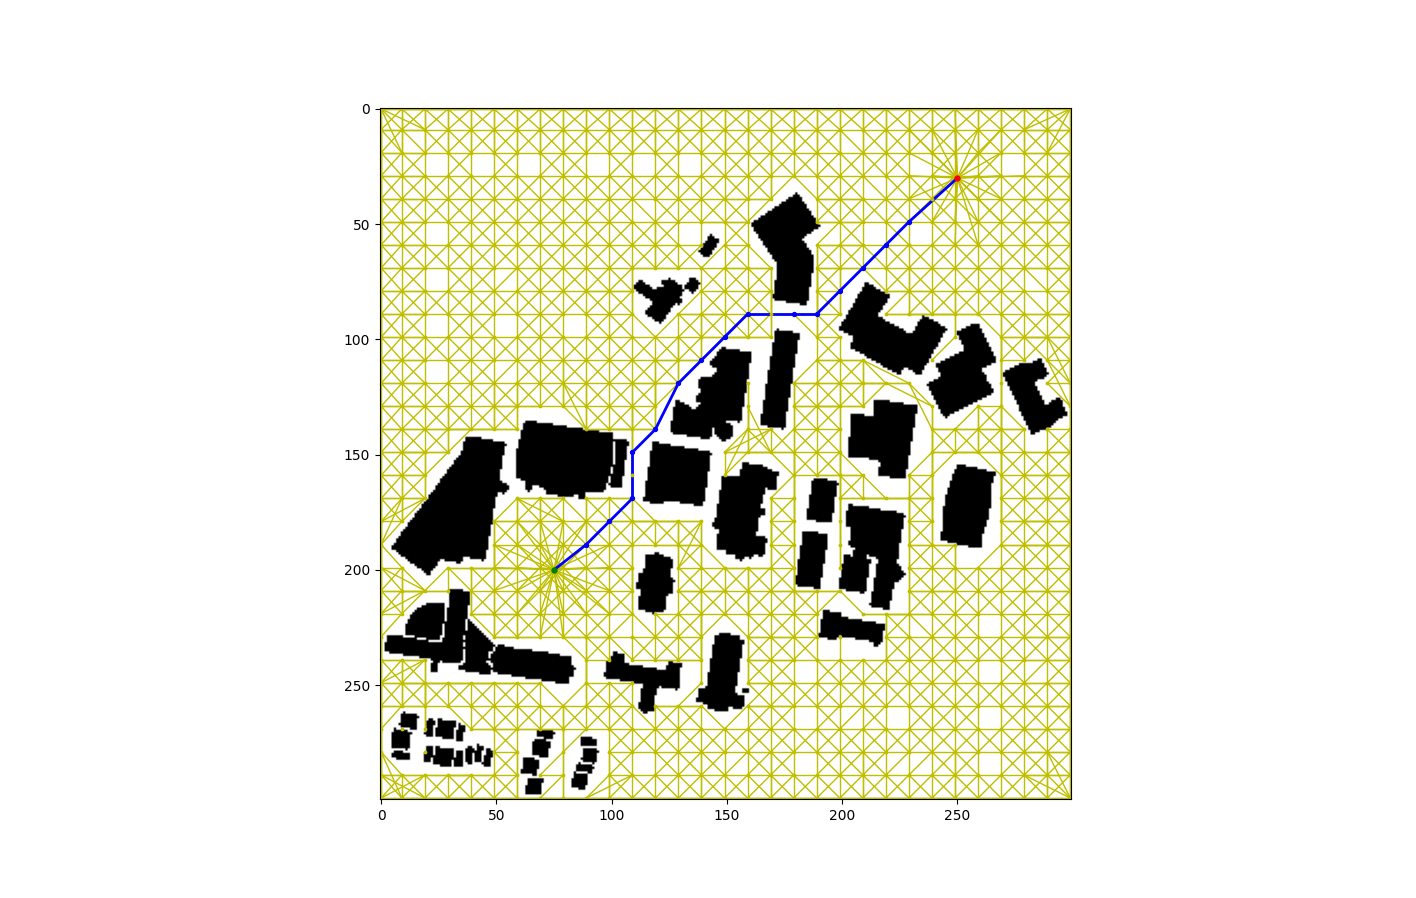
\includegraphics[width=\linewidth]{figures/UniformPRM.png}
        \label{fig:UniformPRM}
        \caption{Uniform Sampling PRM run with 1000 iterations. The graph had 815 nodes and 2971 edges. The length of the path was 260}
    \end{figure} 



    \subsection{Random Sampling PRM}
    \begin{figure}[H]
        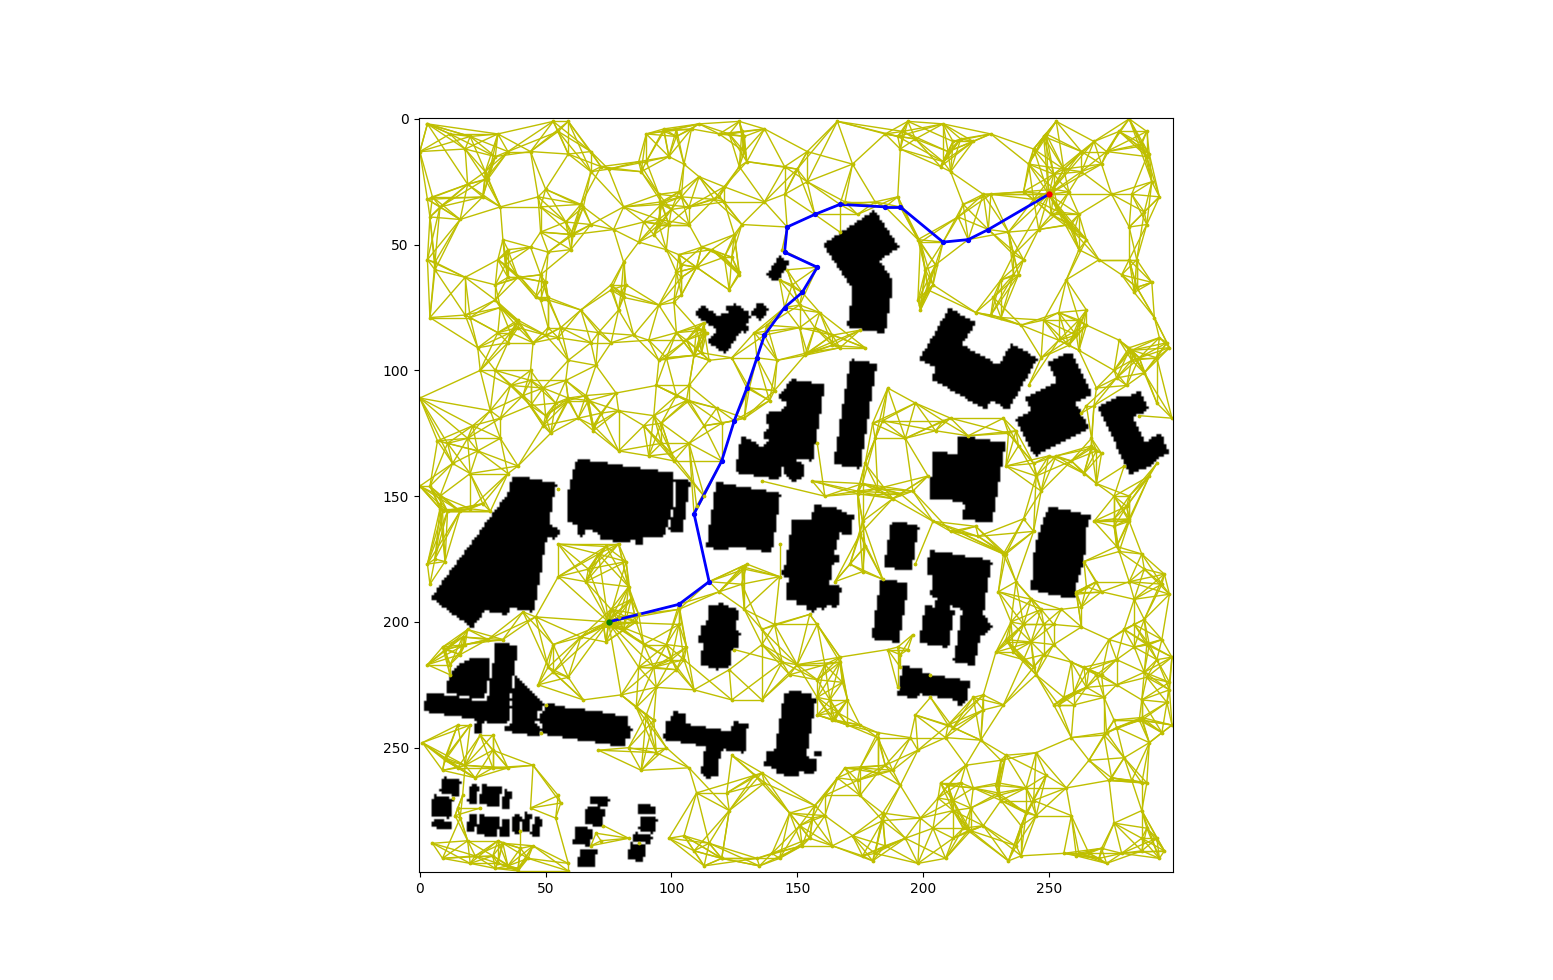
\includegraphics[width=\linewidth]{figures/RandomPRM.png}
        \label{fig:RandomPRM}
        \caption{Random Sampling PRM run with 1000 iterations. The graph had 831 nodes and 3180 edges. The length of the path was 322}
    \end{figure} 

    \subsection{Gaussian Sampling PRM}
    \begin{figure}[H]
        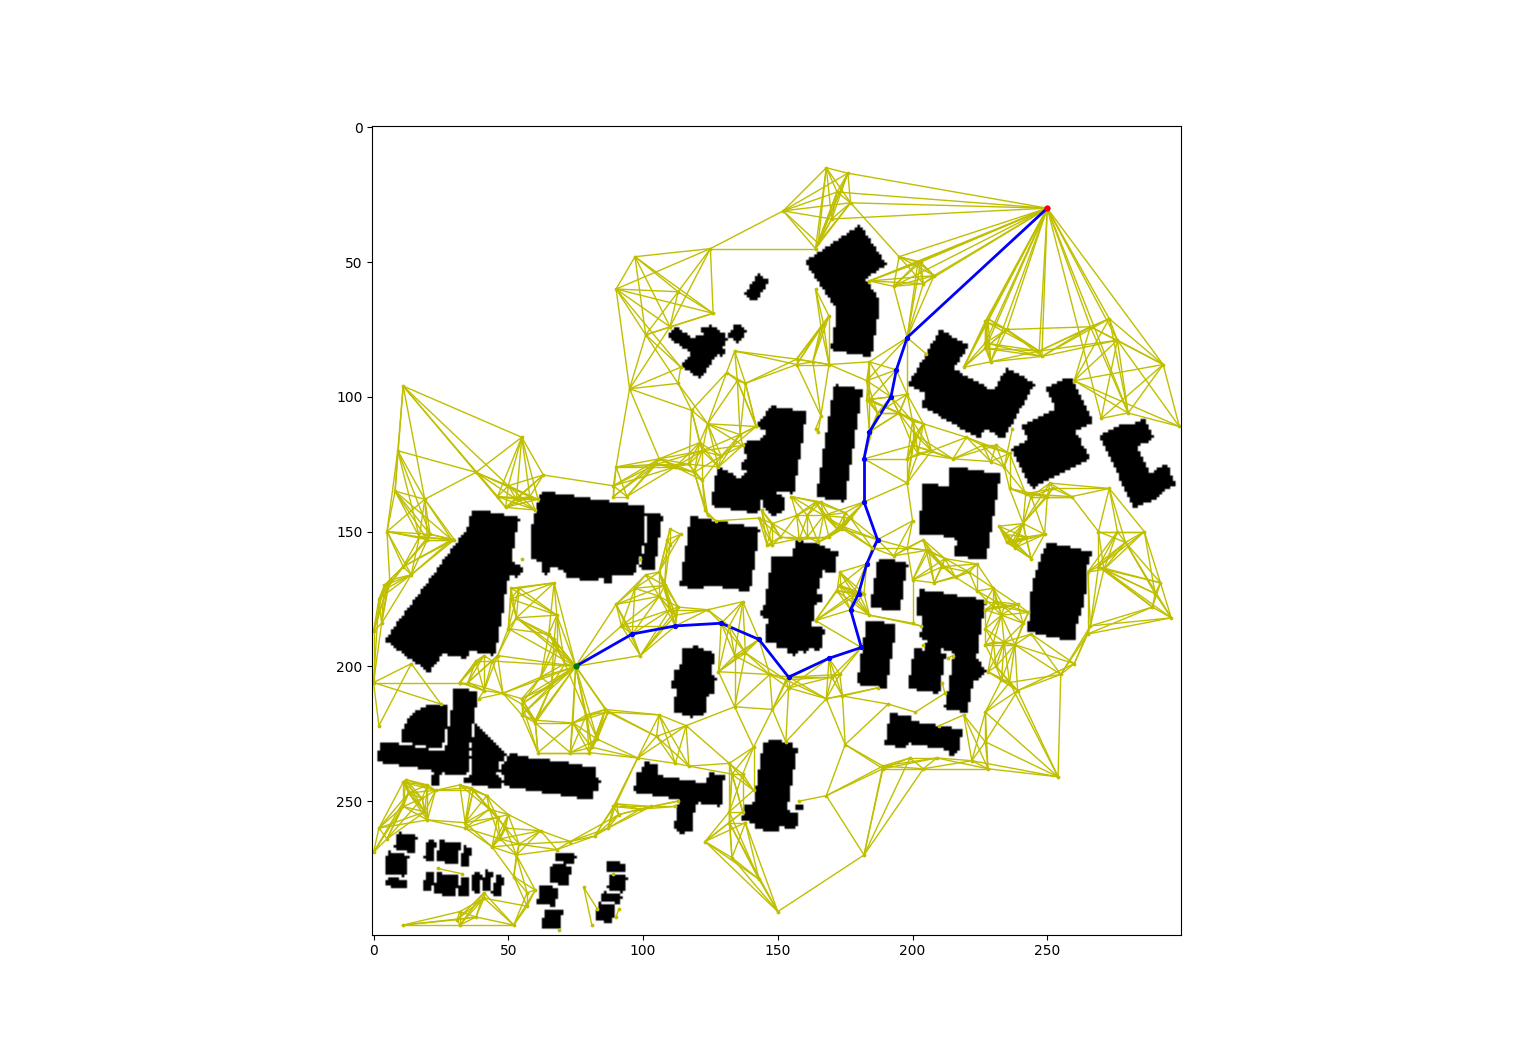
\includegraphics[width=\linewidth]{figures/GaussianPRM.png}
        \label{fig:GaussianPRM}
        \caption{Gaussian Sampling PRM run with 2000 iterations. The graph had 425 nodes and 1474 edges. The length of the path was 312}
    \end{figure} 

    \subsection{Bridge Sampling PRM}
    \begin{figure}[H]
        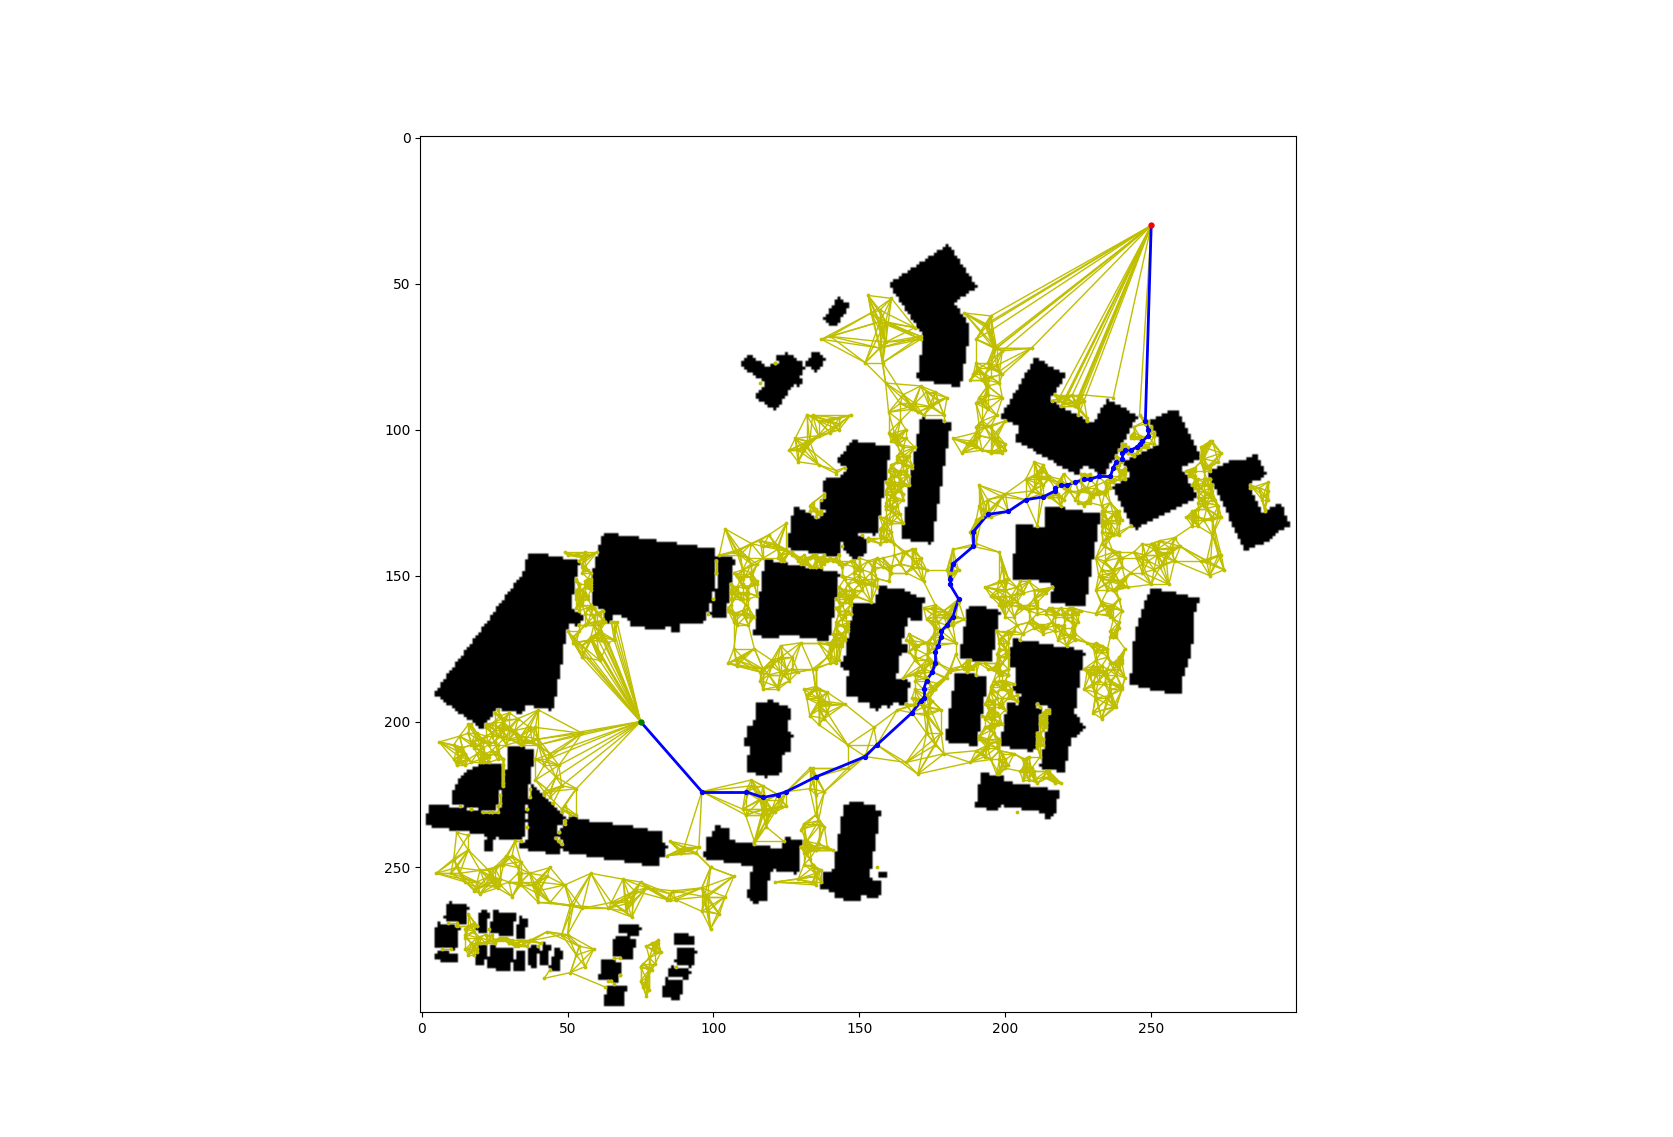
\includegraphics[width=\linewidth]{figures/BridgePRM.png}
        \label{fig:BridgePRM}
        \caption{Bridge Sampling PRM run with 2000 iterations. The graph had 1974 nodes and 7647 edges. The length of the path was 330}
    \end{figure} 

    \subsection{RRT}
    \begin{figure}[H]
        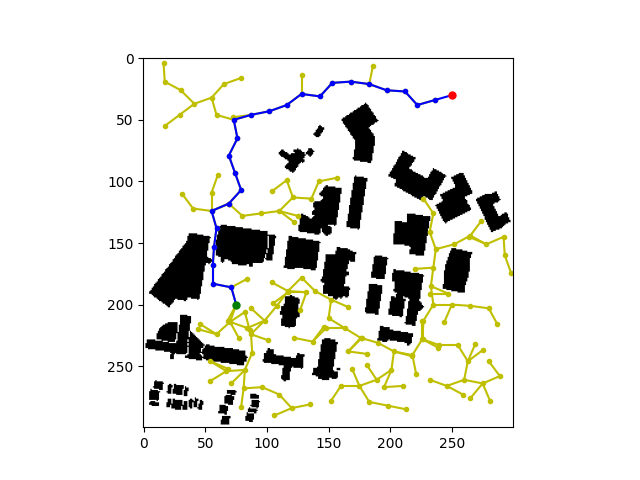
\includegraphics[width=\linewidth]{figures/RRT.png}
        \label{fig:RRT}
        \caption{RRT run with 2000 iterations. It took 161 nodes to find a path length of 374}
    \end{figure}
    
    \subsection{RRT*}
    I did not get a chance to finish my implementation of RRT*. I was having some issues with my rewire function, although it should be the only thing remaining before RRT* implementation works.


    \subsection{Additional Notes and resources}
    I used a few resources. They are cited below:

    Collision checking algorithms: \cite{FastProbabilisticCollisionChecking} \cite{EfficientCollisionChecking}

    RRT and RRT* Resources: \cite{chin_2019} \cite{RRT_RRT-star_Comparison} \cite{Wikipedia_RRT}

    Some additional resources I used: \cite{numpyrandomuniform} \cite{scipyspatialkdtree}

    \newpage

    % References to cite:
    % http://ottelab.com/html_stuff/pdf_files/Bialkowski_WAFR12.pdf
    % https://www.researchgate.net/publication/301796015_Fast_probabilistic_collision_checking_for_sampling-based_motion_planning_using_locality-sensitive_hashing/link/5b0e5755aca2725783f228b4/download
    % Fast Probabilistic Collision Checking forSampling-based Motion Planning usingLocality-Sensitive Hashing
    % https://numpy.org/doc/stable/reference/random/generated/numpy.random.uniform.html
    % https://www.sharpsightlabs.com/blog/np-random-uniform/
    % https://en.wikipedia.org/wiki/Rapidly-exploring_random_tree
    % https://docs.scipy.org/doc/scipy/reference/generated/scipy.spatial.KDTree.html

    % RRT/RRT*
    % https://theclassytim.medium.com/robotic-path-planning-rrt-and-rrt-212319121378
    % https://en.wikipedia.org/wiki/Rapidly-exploring_random_tree

    \printbibliography

\end{document}